\documentclass[tikz,border=4pt]{standalone}
% Estilo común de los diagramas de bloques (se usa con \input en cada standalone)
\usepackage[defaultsans,scale=0.92]{lato}
\usepackage{libertinust1math}
\usepackage{xcolor,amsmath}
\usepackage{tikz}
\usetikzlibrary{positioning,arrows.meta,calc,shapes.geometric}
\usepackage{../../notacion}
\definecolor{ctrlazul}{HTML}{1E5AA8}\definecolor{ctrlnoche}{HTML}{14213D}
\definecolor{ctrlcoral}{HTML}{D1495B}\definecolor{ctrlverde}{HTML}{2A9D8F}
\definecolor{ctrlambar}{HTML}{E09F3E}\definecolor{ctrlgris}{HTML}{5C677D}
\definecolor{ctrlvioleta}{HTML}{6C4AB6}\definecolor{ctrlteal}{HTML}{0F7173}
\tikzset{
  >={Stealth[length=2.4mm]}, every node/.style={font=\small},
  bloque/.style={draw=ctrlnoche,fill=ctrlazul!7,thick,rounded corners=1.5pt,minimum height=9mm,minimum width=13mm,inner sep=4pt},
  suma/.style={draw=ctrlnoche,thick,circle,inner sep=0pt,minimum size=6mm},
  senal/.style={->,thick,draw=ctrlnoche},
  rot/.style={font=\footnotesize,text=ctrlgris},
}

\begin{document}
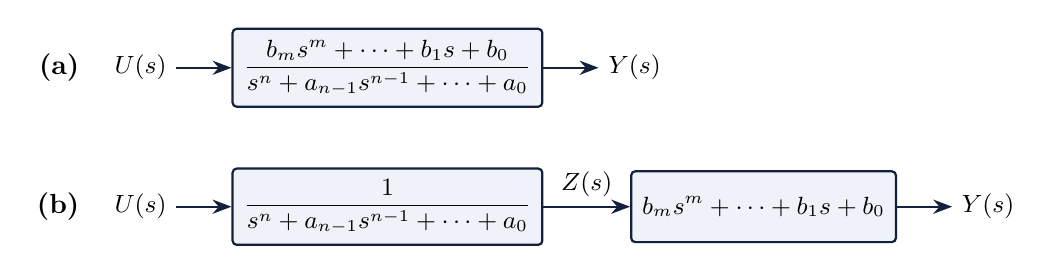
\begin{tikzpicture}
  \node (u) {$U(s)$};
  \node[bloque,right=7mm of u] (g) {$\dfrac{b_ms^m+\dots+b_1s+b_0}{s^n+a_{n-1}s^{n-1}+\dots+a_0}$};
  \node[right=7mm of g] (y) {$Y(s)$};
  \draw[senal] (u)--(g); \draw[senal] (g)--(y);
  \node[left=2mm of u,font=\bfseries] {(a)};
  \node[below=12mm of u] (u2) {$U(s)$};
  \node[bloque,right=7mm of u2] (g1) {$\dfrac{1}{s^n+a_{n-1}s^{n-1}+\dots+a_0}$};
  \node[bloque,right=11mm of g1] (g2) {$b_ms^m+\dots+b_1s+b_0$};
  \node[right=7mm of g2] (y2) {$Y(s)$};
  \draw[senal] (u2)--(g1); \draw[senal] (g1)--node[above]{$Z(s)$}(g2); \draw[senal] (g2)--(y2);
  \node[left=2mm of u2,font=\bfseries] {(b)};
\end{tikzpicture}
\end{document}
